\section{General information}

The project is the making of the course TDT4290 Customer Driven Project. 
Customer driven project is a course held at The Norwegian University of Science and Technology, as mentioned briefly in the preface. 
This course accounts for 15 credits. 
It is a mandatory subject for the 4th year computer science students at IDI. 
The course aims to give the students a real experience with customers in a relevant IT-project. 
This course shall give the students a feel of managing a project in a group. 


All of the different groups is given one customer. 
The customer has put together a project, and to make sure the customer gets what he or she wants, there should be a close relationship with the customer.
Each group also receives an advisor, which will support and give advice to the group. 


The delivery of the course is a report and a product, and this will be presented to an examiner. 
The report is the most important part of the project, and will contain all the documentation for this project. The course will provide realistic experience in both report writing and product development driven by a customer. 
This will help the students perform better when they are out in real life employment situations.

\section{Structure of report}
\begin{tabular}{l|p{10cm}}
\textbf{Chapter} & \textbf{Description} \\
\hline
Chapter 1 & The introduction chapter introduces the problem, and introduces the members and stakeholders of this project.
This chapter also explains the motivation and goals. \\
\hline
Chapter 2 &  The preliminary Study chapter describes the work and research done. This chapter describes alternative solutions, and an evaluation these solutions. \\
\hline
Chapter 3 &  The planning chapter describes the project plan, the organization, quality assurance and planned workload.  \\
\hline
Chapter 4 &  The requirements chapter describes the requirements, both functional and non-functional. It also describes Use cases for the system. \\
\hline
Chapter 5 &  The test plan chapter contains the approach for testing with the overall test plan for the project.\\
\hline
Chapter 6	 &  The architecture chapter explains the structure of the system, and how it is put together. \\
\hline
Chapter 7	 &   The tools and strategy chapter describes the different tools we chose to use for this project.\\
\hline
Chapter 8-14 	&  In the sprint chapters the reader can see how the product has developed during the time of the project. This includes planning, architecture, the implementation, testing and evaluation of the sprint. \\
\hline
Chapter 15 	 &  The testing chapter describes the different tests. Everything from unit testing to acceptance testing. \\
\hline
Chapter 16 	 &  Evaluation chapter includes the team dynamics, risk evaluation, an evaluation of the customer, supervisor and of course the task. \\
\hline
Chapter 17 	 &  Conclusion chapter sums up the project, and discusses the solution, and looks at further work. \\
\hline
Chapter 18 	 &  The referances chapter contains references. \\
\hline
Chapter 19 	 &  This chapter contains attachments. \\
\hline
Appendix 	 &   The appendix contains user manual, installation guide, meeting minutes and more.\\

\hline
\end{tabular}
\section {Terminology}
\section{Project and project name}

The customer wants a product to make the audience as a screen on a rock concert. We decided to name the product "digital lighter". We agreed on this name because this product digitalizes the concept from "the old days", where the crowd at a concert held up lighters, to create a special atmosphere. 

\section{Project purpose and concept}

The audience members at a rock concert should be able to download a simple application to their cell phone, and register this through a simple GUI.
Behind the artist on stage there is a screen, with a simple camera on top. 
The camera is taking pictures of the audience. 
At special occasions the audience will be instructed, by the artist, to hold up their phones with the screen towards the stage. 
The mobile is a replacement for the lighter.  

On control a signal the application will fill the entire mobile screen with a single color.
The control signal can as an example say: " all pixels white". 
The signal will be specific for each application.
Each mobile will be a pixel in a larger picture, which will be presented on the big screen. 
What kind of picture the audience can create will depend on the number of people in the audience.   

As a motivation for the audience to hold up their phone, the camera on top of the screen will take pictures of the audience.
In that way the audience can see a reflection of them selves, and see what kind of picture they are creating together.

\section{Project goal}

\section{Stakeholders}

The stakeholders in this project is any person or organization, which has some interest or is affected by this project. Together they construct the different restrictions and goals for the project. 
You can see the organization chart in figure \ref{img:organization_chart}.

\begin{figure}[h]
    \begin{center}
    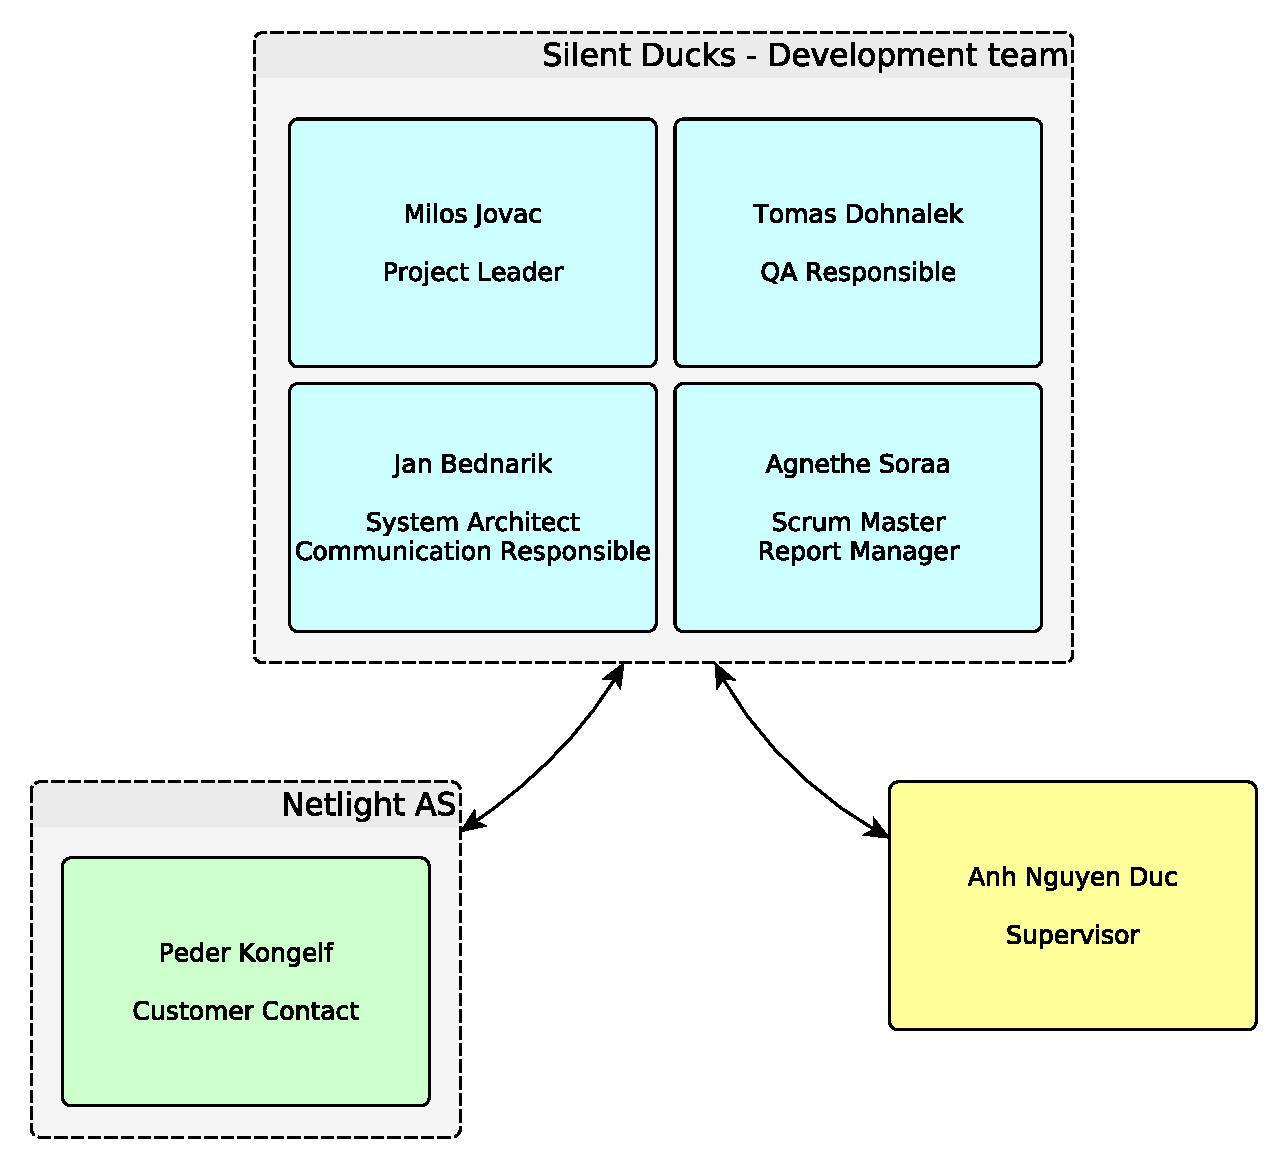
\includegraphics[scale=0.4]{images/organization_chart.pdf}
    \label{img:organization_chart}
    \caption{Chart depicting team organization and its stakeholders.}
    \end{center}
\end{figure}

\subsection{Customer}
Netlight AS is a consulting company engaged in IT and management. Their field of expertise is within IT management, IT governance, IT-strategy, IT-organization and IT-research. They deliver unique solutions based on their customers requirements. They operates throughout Europe with offices in Stockholm, Oslo, London, Munich and Helsinki. The company was founded at 1999 and employs to 500 employees. 
\subsubsection{Customer contact}
Peder Kongelf will be our contact person in Netlight. We will have weekly meetings with him to make sure the project is going in the right direction, and of course get opportunities to ask questions. This way we will get a better understanding of the project.

\subsection{Development team}
 The development team's role is, first of all, to meet all requirements presented by the customer and IDI. We are responsible for development of the project. We are also responsible for writing all the documentation for this course.  Our interest in the project is to receive experience with new technologies and project management, as well as to receive satisfactory grading. The project was intended for 5-7 students,but we are only 4 members in our team. This will, in some way, affect what the team can manage towards what was expected when the project was put together.

\subsection{Supervisor}

Anh Nguyen Doc

\subsubsection{NTNU and IDI}

\subsection{End users}
Is a everyday person who uses the end product. Our plan is to release the product on the application store for Android. That way we can get feedback from someone other than supervisor and customer. 
\subsection{Stakeholder summary}
\begin{tabular}{l|l|l}
\textbf{Person} & \textbf{Email} & \textbf{Role}\\
\hline
Milos Jovac &  milosjovac@gmail.com & Team member  \\
Jan Bednarik2 &  ja.bedna1@gmail.com & Team member\\
Agnethe Soraa & agnethes0raa@gmail.com & Team member  \\
Tomas Dohnalek & dohnto@gmail.com & Team member \\
\hline
Peder Kongelf & peder.kongelf@gmail.com  & Customer\\
\hline
Anh Nguyen Doc	 & anhn@idi.ntnu.no & Supervisor \\
\hline

\end{tabular}

\section{Project background}